\section{Considerações iniciais}

O processo de manipular imagens para que elas se tornem mais satisfatórias para um determinado objetivo depende do domínio de aplicação. Ou seja, não existe uma teoria geral para melhorar qualquer tipo de imagem \cite{Gonzalez2007}: um método que processa melhor uma imagem bem definida por suas cores difere do processamento de imagens texturizadas, às quais um processamento sobre a intensidade dos pixels da imagem -- como uma operação de borramento -- pode ocasionar perda da textura. Assim, justifica-se a exploração de um vasto número de métodos de processamento de imagens e bases.

Nesta pesquisa, oito métodos de processamento de imagens são aplicados nas imagens minoritárias originais, gerando imagens artificiais a partir dessas. Isso é realizado a fim de permitir a extração de informações latentes com o objetivo de melhorar a classificação com alguma técnica de Aprendizado de Máquina, o que reflete a melhora da diferenciação entre as classes. Dada a quantidade de imagens necessárias para rebalancear a base original, são geradas imagens utilizando cada um dos métodos, além de uma versão combinando todos eles (ou seja, compondo um conjunto com algumas imagens processadas por cada método) e outra apenas replicando as imagens como \textit{baseline}. Como demonstrado na Figura~\ref{fig:escolha}, dado o conjunto de treinamento da classe (ou classes) com menor número total de imagens, é realizado o rebalanceamento ao aplicar os métodos descritos neste capítulo e posteriormente essas imagens resultantes são utilizadas como treinamento.

Os métodos de geração artificial para o rebalanceamento de classes de imagens são descritos neste capítulo. Os experimentos posteriormente destacados no Capítulo~\ref{cap:resultados-geracao} foram realizados utilizando as operações de: borramento; mistura ponderada; \textit{unsharp masking}; composição; combinação de \textit{thresholds}; combinação com saliência; SMOTE visual; e adição de ruído.

\begin{figure}[!htbp]
  \begin{center}
    \includegraphics[width=0.7\linewidth]{\detokenize {figuras/rebalance.pdf}}
  \end{center}
  \caption[Geração artificial da classe minoritária para rebalancear as classes. Para cada imagem necessária para igualar o número de imagens da base, $1 \leq n \leq 16$ imagens originais são dadas como entrada para uma operação de geração artificial. A nova imagem é utilizada como treinamento da base.]{Geração artificial da classe minoritária para rebalancear as classes. Para cada imagem necessária para igualar o número de imagens da base, $1 \leq n \leq 16$ imagens originais são dadas como entrada para uma operação de geração artificial. A nova imagem é utilizada como treinamento da base. \textit{Fonte: Elaborado pela autora.}}
  \label{fig:escolha}
\end{figure}


%  \begin{figure}[hbpt]
%  \begin{center}
%    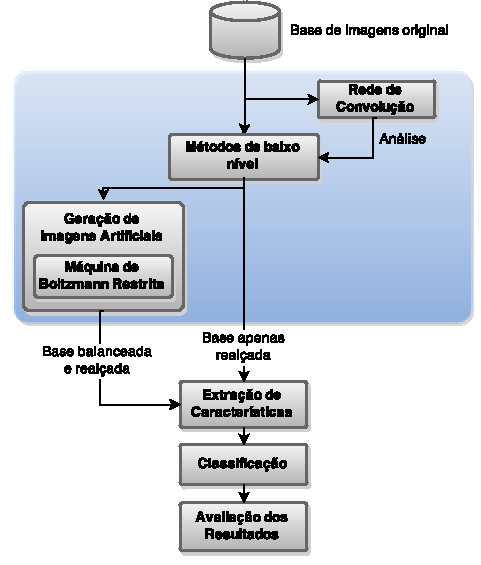
\includegraphics[width=1\linewidth]{\detokenize {figuras/geral.pdf}}
%  \end{center}
%   \caption[]{\textit{Fonte: Elaborado pela autora.}}
%  \label{fig:escolha}
% \end{figure}

% As etapas para a geração das imagens artificiais, passo \ref{item} da seção anterior, foram:
%
% \begin{enumerate}
% \item Selecionar uma imagem aleatoriamente do conjunto de treino;
% \item Selecionar uma operação aleatória entre: borramento, adição de ruído, \textit{unsharp mask}, mistura ou composição;
% \begin{enumerate}
% \item Caso seja selecionada a composição: encontrar uma outra imagem aleatória, selecionar um quadrante dessa imagem e novamente uma operação entre: borramento, adição de ruído, \textit{unsharp mask} ou mistura;
% \end{enumerate}
% \item Aplicar essa operação na imagem previamente selecionada e adicionar essa imagem gerada ao conjunto de treino;
% \item Repetir os passos 2 a 4 até que as classes estejam igualmente balanceadas.
% \end{enumerate}

%%%%%%%%%%%%%%%%%%%%%%%%%%%%%%%%%%%%%%%%%%%%%%%%%%%%%%%%%%%%%%%%%%%%%%%%%%%%%%%%
\section{Borramento}

Também conhecido como filtro de suavização, o borramento é uma operação de processamento comumente utilizada com o objetivo de filtrar uma imagem, removendo ruídos e detalhes não relevantes. Normalmente esse tipo de filtro provoca também um certo borramento das bordas, como pode ser observado na Figura~\ref{fig:blur}. Esse comportamento não é esperado quando queremos gerar novas imagens, pois informações relevantes podem ser removidas. Com o intuito de preservar as bordas, a operação de borramento \textbf{filtro bilateral} pode ser utilizada. Ela substitui o valor do pixel $I(x,y)$ pela média dos pixels vizinhos de intensidade similar \cite{Tomasi1998}. Ou seja, é uma média ponderada das intensidades que considera a diferença dos valores entre vizinhos para preservar bordas. Assim, para um pixel influenciar outro, deve estar próximo no espaço de coordenadas e possuir intensidade similar. O Algoritmo~\ref{alg:blur} descreve os passos desse filtro na sua versão mais simples, de força bruta. Considere $W$ o termo de normalização, e $G$ o filtro de Gaussianas. A Figura~\ref{fig:gen:blur} exemplifica o seu funcionamento: à esquerda está demonstrada a imagem original e à direita a imagem borrada.

\begin{figure}[!htbp]
  \begin{center}
    \subfloat[Original]{
      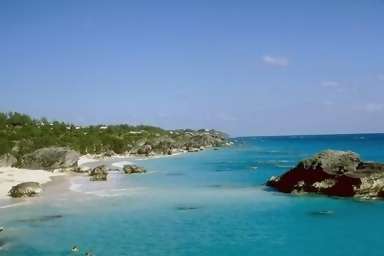
\includegraphics[width=.4\linewidth]{\detokenize{figuras/geracao/blur-a.png}}
    }
    \hspace{0.1\textwidth}
    \subfloat[Imagem artificial]{
      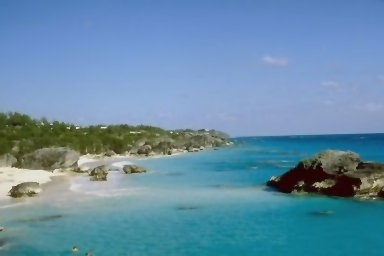
\includegraphics[width=.4\linewidth]{\detokenize{figuras/geracao/blur-b.png}}
    }
  \end{center}
  \caption[Geração artificial utilizando borramento com filtro bilateral.]{Geração artificial utilizando borramento com filtro bilateral. \textit{Fonte:~Elaborado pela autora.}}
  \label{fig:gen:blur}
\end{figure}

\vspace{0.5cm}
\begin{algorithm}[!htbp]
  \caption{Geração artificial: borramento com filtro bilateral}
  \label{alg:blur}
  \SetAlgoLined
  \Entrada{
  \begin{itemize}
    \item[] Imagem colorida $I_{original}$ em formato RGB
    % \item[] Diâmetro $d$ de vizinhança de pixels
    \item[] Sigma do espaço de cor $\sigma_{range}$
    \item[] Sigma do espaço de coordenadas $\sigma_{spatial}$
  \end{itemize}
  }
  \Saida{
  \begin{itemize}
    \item[] Imagem borrada $I_{borrada}$
  \end{itemize}
  }
  \ParaCada{pixel $(x,y)$}{
    $I_{borrada}(x,y) \gets 0$\;
    $W(x,y) \gets 0$\;

    \ParaCada{pixel $(i,j)$}{
      $w \gets G_{\sigma_{spatial}} (\lVert(x,y) - (i,j)\rVert) G_{\sigma_{range}} (\lvert I_{original}(x,y) - I_{original}(i,j) \rvert) $\;
      $I_{borrada}(x,y) \gets I_{borrada}(x,y) + w I_{original}(i,j)$\;
      $W(x,y) \gets W(x,y) + w$\;
    }
    $I_{borrada}(x,y) \gets I_{borrada}(x,y) / W(x,y)$\;
  }
\end{algorithm}
\vspace{0.5cm}

\FloatBarrier
\begin{description}
  \item[Parâmetros e suas variações] Conforme descrito no Algoritmo~\ref{alg:blur}, os parâmetros para essa geração são: o $\sigma_{range}$ do espaço de cor e o $\sigma_{spatial}$ do espaço de coordenadas. Esses parâmetros dependem das propriedades das imagens e dos resultados pretendidos. Quanto maior o $\sigma_{range}$, mais próximo da convolução Gaussiana e assim ocorre o borramento de intensidades mais distintas. Já o $\sigma_{spatial}$ controla o tamanho da vizinhança. Dessa forma, esses valores são escolhidos arbitrariamente para cada aplicação específica \cite{Tomasi1998}. Como o nosso objetivo com a geração das imagens não foi especializar no comportamento de uma classe de imagens, um valor foi escolhido aleatoriamente, e a partir dele os parâmetros de entrada foram definidos.

  \item[Limitações] Esse filtro tende a remover texturas e criar novos contornos. Dependendo dos valores, pode gerar uma imagem ``cartoonizada''.

  \item[Métodos relacionados] São diversos os métodos de borramento descritos na literatura, como a filtragem Gaussiana e as filtragens de medianas e médias.

  % \item[Visualização] É interessante notar na Figura \ref{vis:blur} o comportamento da adição de imagens borradas para o rebalanceamento de classes bem descritas pela propriedade da cor.

\end{description}
%%%%%%%%%%%%%%%%%%%%%%%%%%%%%%%%%%%%%%%%%%%%%%%%%%%%%%%%%%%%%%%%%%%%%%%%%%%%%%%%
\section{Aguçamento}

Diferente da suavização, o processamento de aguçamento procura enfatizar as transições de intensidade. Um método bem conhecido para atingir tal objetivo é o \textit{unsharp mask}. Ele borra a imagem, subtrai a imagem borrada da original e adiciona essa diferença na imagem original, dado um peso $k$ (ver Algoritmo \ref{alg:unsharp}). A imagem resultante, ilustrada na Figura~\ref{fig:gen:unsharp}, é uma versão realçada da imagem original. Isso porque adiciona à imagem justamente o que é removido com um filtro de suavização.

\vspace{0.5cm}
\begin{algorithm}[!htbp]
  \caption{Geração artificial: aguçamento}
  \label{alg:unsharp}
  \SetAlgoLined
  \Entrada{
  \begin{itemize}
    \item[] Imagem colorida $I_{\textit{original}}$ em formato RGB
  \end{itemize}
  }
  \Saida{
  \begin{itemize}
    \item[] Imagem aguçada $I_{\textit{aguçada}}$\\
  \end{itemize}
  }
  $I_{\textit{borrada}} \gets \textit{filtro\_de\_suavização}(I_{\textit{original}})$

  \ParaCada{pixel $(x,y)$ em $I_{\textit{original}}$}{
  $I_{\textit{diferença}} \gets I_{\textit{original}}(x,y) - I_{\textit{borrada}}(x,y)$\;
  $I_{\textit{aguçada}}(x,y) \gets I_{\textit{original}}(x,y) + k*I_{\textit{diferença}}$\;
  }
\end{algorithm}
\vspace{0.5cm}

\begin{figure}[!htbp]
  \begin{center}
    \subfloat[Original]{
      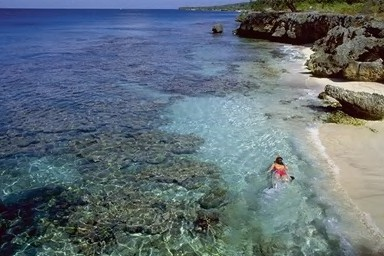
\includegraphics[width=.4\linewidth]{\detokenize{figuras/geracao/unsharp-a.png}}
    }
    \hspace{0.1\textwidth}
    \subfloat[Imagem artificial]{
      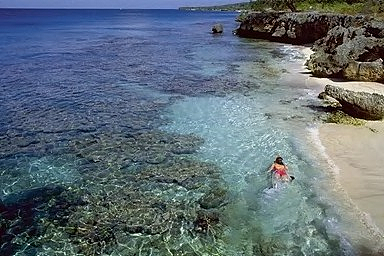
\includegraphics[width=.4\linewidth]{\detokenize{figuras/geracao/unsharp-b.png}}
    }
  \end{center}
  \caption[Geração artificial utilizando \textit{unsharp masking}.]{Geração artificial utilizando \textit{unsharp masking}. \textit{Fonte:~Elaborado pela autora.}}
  \label{fig:gen:unsharp}
\end{figure}

\begin{description}
  \item[Parâmetros e suas variações] Pode-se variar o parâmetro $k$ de forma a ponderar a soma dessa diferença. Para a geração das imagens da classe minoritária, foi utilizado $k = 1$.

  \item[Limitações] É possível que existam pixels com valor negativo no resultado final. Isso pode causar o aparecimento de uma áurea em volta das bordas, efeito não desejado \cite{Gonzalez2007}.

  \item[Métodos relacionados] Outros algoritmos de aguçamento conhecidos são: utilizar primeira derivada (grandiente), ou a segunda derivada da imagem (Laplaciano).

  % \item[Visualização]
\end{description}
%%%%%%%%%%%%%%%%%%%%%%%%%%%%%%%%%%%%%%%%%%%%%%%%%%%%%%%%%%%%%%%%%%%%%%%%%%%%%%%%
\section{Adição de ruído}

O ruído de Poisson ocorre na contagem de fótons de dispositivos ópticos. Ele segue a distribuição de Poisson, que representa o número de ocorrências de um evento em um dado instante de tempo \cite{knuth} (knuth vem aqui :-)). O efeito da adição de ruído pode ser visto na Figura~\ref{fig:gen:noise}.

\begin{figure}[!htbp]
  \begin{center}
    \subfloat[Original]{
      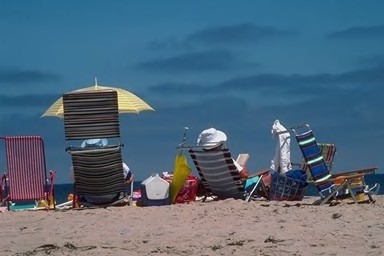
\includegraphics[width=.4\linewidth]{\detokenize{figuras/geracao/noise-a.png}}
    }
    \hspace{0.1\textwidth}
    \subfloat[Imagem artificial]{
      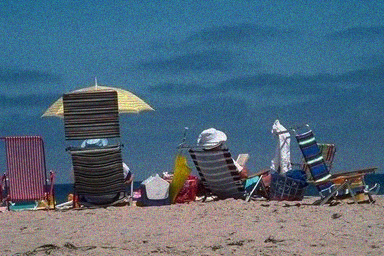
\includegraphics[width=.4\linewidth]{\detokenize{figuras/geracao/noise-b.png}}
    }
  \end{center}
  \caption[Geração artificial utilizando adição de ruído de Poisson.]{Geração artificial utilizando adição de ruído de Poisson. \textit{Fonte:~Elaborado pela autora.}}
  \label{fig:gen:noise}
\end{figure}

% A distribuição de Poisson segue a equação:
% \begin{equation}
% $P_\mu)(n) = (e^(-\mu)\mu^(n))/(n!), n >= 0$
% \end{equation}

Uma possível implementação para encontrar os valores de Poisson foi desenvolvida por Knuth e pode ser vista no Algoritmo~\ref{alg:noise}. A diferença do cálculo da distribuição de Poisson para sua adição em uma imagem, é que para calcular o valor de ruído em um pixel, esse pixel é considerado a média dessa distribuição. Ou seja, $\mu \equiv I_{original}(x,y)$. Para intensidades próximas a zero, o limite será $L \approx 1$ e, portanto, a probabilidade $p$ estará muito próxima do limite e o contador $k$ terá um valor baixo. Dessa forma, para intensidades escuras haverá pouco ruído. Por outro lado, em intensidades próximas a 255, $p \approx 0$. Assim, são necessárias muitas interações até $p > L$ e maior será a intensidade resultante $k-1$.

\vspace{0.5cm}
\begin{algorithm}[!htbp]
  \caption{Geração artificial: ruído de Poisson}
  \label{alg:noise}
  \SetAlgoLined
  \Entrada{
  \begin{itemize}
    \item[] Imagem colorida $I_{original}$ em formato RGB
  \end{itemize}
  }
  \Saida{
  \begin{itemize}
    \item[] Imagem ruidosa $I_{ruidosa}$\\
  \end{itemize}
  }

  \ParaCada{canal de cor}{
    \ParaCada{pixel $(x,y)$}{
    $L \gets exp(-I_{original}(x,y))$\;
    $p \gets 1$\;
    $k \gets 0$\;
    \DoWhile{$p > L$}{
    $k \gets k + 1$\;
    $p \gets p * \text{número aleatório uniforme entre 0 e 1}$\;
    }
    $I_{ruidosa}(x,y) \gets k - 1$\;
    }
  }
\end{algorithm}
\vspace{0.5cm}

\begin{description}
  \item[Parâmetros e suas variações] Para a adição desse ruído em uma imagem, não é fornecido nenhum parâmetro. O ruído é calculado para cada pixel.
  \item[Limitações] A adição de ruído é normalmente indesejável. Porém, a utilizamos para englobar um processamento de imagens que, de certa forma, se contrapõe ao borramento.
  \item[Métodos relacionados] Esse método está relacionado com diversos outros ruídos, como o sal e pimenta, por exemplo.
  % \item[Visualização]
\end{description}
%%%%%%%%%%%%%%%%%%%%%%%%%%%%%%%%%%%%%%%%%%%%%%%%%%%%%%%%%%%%%%%%%%%%%%%%%%%%%%%%
\section{SMOTE visual}

Conforme visto na Seção \ref{sec:smote}, o SMOTE é um método de rebalanceamento aplicado após a extração de características. É proposta uma alternativa, chamada de SMOTE visual, onde imita-se o funcionamento do SMOTE, porém no nível de pixels. A diferença é que não é feito entre as imagens mais próximas, mas sim entre duas imagens escolhidas de forma aleatória do conjunto de treinamento da classe minoritária.

Para cada pixel é calculado a diferença entre as duas imagens. Essa diferença é então multiplicada por um número aleatório no intervalo $[0-1]$ e adicionado
na imagem original (ver Algoritmo~\ref{alg:smotevisual}). O efeito que esse processamento causa na imagem pode ser visualizado na Figura~\ref{fig:gen:smotevisual}.

\vspace{0.5cm}
\begin{algorithm}[!htbp]
  \caption{Geração artificial: SMOTE visual}
  \label{alg:smotevisual}
  \SetAlgoLined
  \Entrada{
  \begin{itemize}
    \item[] Imagem colorida $I_{original}$ em formato RGB
    \item[] Imagem colorida $I_{\textit{segunda\_original}}$ em formato RGB
  \end{itemize}
  }

  \Saida{
  \begin{itemize}
    \item[] Imagem gerada $I_{gerada}$\\
  \end{itemize}
  }

  \ParaCada{pixel $(x,y)$} {
  $\textit{diferença} \gets I_{original}(x,y) - I_{\textit{segunda\_original}}(x,y)$\;
  $\text{gap} \gets \text{número aleatório entre 0 e 1}$\;
  $I_{gerada}(x,y) \gets I_{original}(x,y) + gap*\textit{diferença}$\;
  }

  $\textit{mínimo} \gets \textit{menor valor}(I_{gerada})$\;

  $\textit{máximo} \gets \textit{maior valor}(I_{gerada})$\;

  \ParaCada{pixel $(x,y)$} {
  $I_{gerada}(x,y) \gets I_{gerada}(x,y) - \textit{mínimo}$\;
  }

  \ParaCada{pixel $(x,y)$} {
  $I_{gerada}(x,y) \gets I_{gerada}(x,y) * (255/(\textit{máximo} - \textit{mínimo}))$\;
  }
\end{algorithm}
\vspace{0.5cm}

\begin{figure}[!htbp]
  \begin{center}
    \begin{center}
    \subfloat[Original]{
      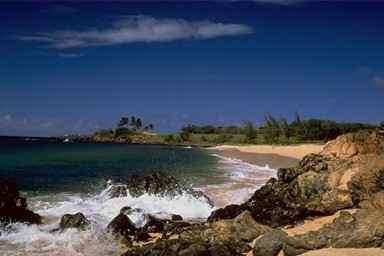
\includegraphics[width=.3\linewidth]{\detokenize{figuras/geracao/smote-a.png}}
    }
    \subfloat[Original]{
      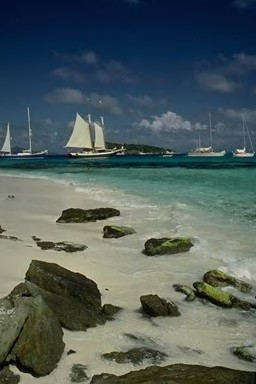
\includegraphics[width=0.2\linewidth]{\detokenize{figuras/geracao/smote-b.png}}
    }
  \end{center}
    \subfloat[Imagem artificial]{
      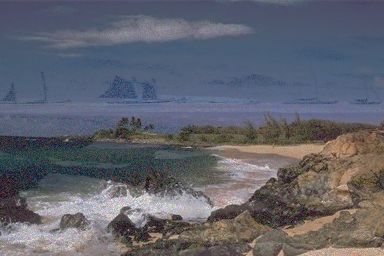
\includegraphics[width=.5\linewidth]{\detokenize{figuras/geracao/smote-c.png}}
    }
  \end{center}
  \caption[Geração artificial utilizando o método SMOTE no espaço visual.]{Geração artificial utilizando o método SMOTE no espaço visual. \textit{Fonte:~Elaborado pela autora.}}
  \label{fig:gen:smotevisual}
\end{figure}

\begin{description}
  \item[Limitações] Esse método adiciona texturas e bordas que não estavam originalmente nas imagens.

  \item[Métodos relacionados] Esse método é visualmente parecido com o de mistura ponderada, apresentado na próxima seção.

  % \item[Visualização]
\end{description}
%%%%%%%%%%%%%%%%%%%%%%%%%%%%%%%%%%%%%%%%%%%%%%%%%%%%%%%%%%%%%%%%%%%%%%%%%%%%%%%%
\section{Mistura ponderada}

Essa geração calcula a soma ponderada de duas imagens, de acordo com o
Algoritmo~\ref{alg:blend}. O efeito dessa mistura pode ser visto na Figura~\ref{fig:gen:blend}, onde dadas duas imagens como entrada, a imagem da direita corresponde à soma delas.

\begin{algorithm}[!htbp]
  \vspace{0.5cm}
  \caption{Geração artificial: mistura ponderada}
  \label{alg:blend}
  \SetAlgoLined
  \Entrada{
    \begin{itemize}
      \item[] Primeira imagem colorida $I$ em formato RGB
      \item[] Segunda imagem colorida $I_2$ em formato RGB
    \end{itemize}
  }
  \Saida{Imagem gerada $G$}

  {$\alpha \gets \text{número aleatório entre 10 e 80}$\;}
  {$\beta \gets 100 - \alpha$\;}

  \ParaCada{pixel $(x,y)$} {
  $\text{G}(x,y) \gets \beta.I(x,y) + \alpha.I_2(x,y)$\;
  }
\end{algorithm}
\vspace{0.5cm}

\begin{figure}[!htbp]
  \begin{center}
    \subfloat[Original]{
      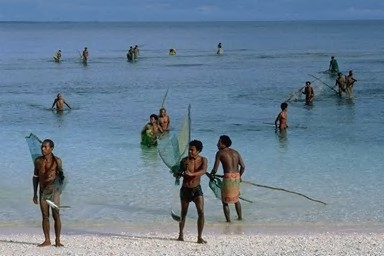
\includegraphics[width=.3\linewidth]{\detokenize{figuras/geracao/blend-a.png}}
    }
    \subfloat[Original]{
      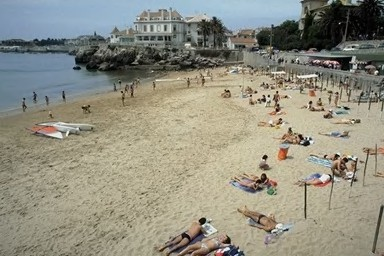
\includegraphics[width=0.3\linewidth]{\detokenize{figuras/geracao/blend-b.png}}
    }
    \subfloat[Imagem artificial]{
      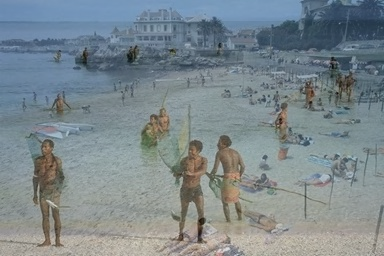
\includegraphics[width=.3\linewidth]{\detokenize{figuras/geracao/blend-c.png}}
    }
  \end{center}
  \caption[Geração artificial utilizando uma mistura ponderada de duas imagens.]{Geração artificial utilizando uma mistura ponderada de duas imagens. \textit{Fonte:~Elaborado pela autora.}}
  \label{fig:gen:blend}
\end{figure}

\begin{description}
  \item[Parâmetros e suas variações] Os parâmetros $\alpha$ e $\beta$ são escolhidos de forma aleatória. Um valor entre 10\% e 80\% é escolhido para $\alpha$; e $\beta$ equivale ao valor restante para completar 100\%.

  \item[Limitações] Assim como todas as gerações artificiais que envolvem a mistura de imagens, efeitos são adicionados às imagens originais. Dependendo da combinação dos métodos de descrição, quantização e classificação, isso pode piorar a acurácia da classificação.

  \item[Métodos relacionados] É um método de combinação de imagens primitivo. Algoritmos similares são muito mais complexos, como os de \textit{threshold} e saliência descritos a seguir.

  % \item[Visualização]

\end{description}
%%%%%%%%%%%%%%%%%%%%%%%%%%%%%%%%%%%%%%%%%%%%%%%%%%%%%%%%%%%%%%%%%%%%%%%%%%%%%%%%
\section{Mistura limiarizada}

A combinação de \textit{thresholds} é uma composição do fundo (\textit{background}) de uma imagem e do objeto da cena (\textit{foreground}) de outra imagem. A Figura~\ref{fig:gen:threshold} mostra a mistura dos \textit{thresholds} de duas imagens originais para compor uma nova imagem. O Algoritmo~\ref{alg:threshold} descreve as operações necessárias para realizar tal processamento.

\begin{figure}[!htbp]
  \begin{center}
    \subfloat[Original]{
      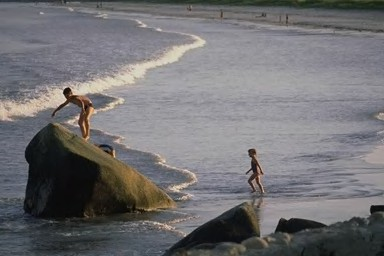
\includegraphics[width=.3\linewidth]{\detokenize{figuras/geracao/threshold-a.png}}
    }
    \subfloat[Original]{
      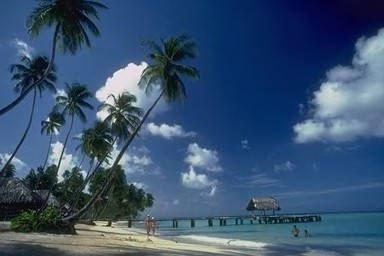
\includegraphics[width=0.3\linewidth]{\detokenize{figuras/geracao/threshold-b.png}}
    }
    \subfloat[Imagem artificial]{
      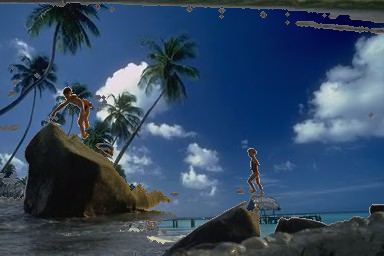
\includegraphics[width=.3\linewidth]{\detokenize{figuras/geracao/threshold-c.png}}
    }
  \end{center}
  \caption[Geração artificial utilizando uma mistura limiarizada de duas imagens.]{Geração artificial utilizando uma mistura limiarizada de duas imagens. \textit{Fonte:~Elaborado pela autora.}}
  \label{fig:gen:threshold}
\end{figure}

\vspace{0.5cm}
\begin{algorithm}[!htbp]
  \caption{Geração artificial: mistura limiarizada}
  \label{alg:threshold}
  \SetAlgoLined
  \Entrada{
    \begin{itemize}
      \item[] Imagem colorida $I$ em formato RGB
      \item[] Imagem colorida $I_2$ em formato RGB
    \end{itemize}
  }
  \Saida{Imagem gerada $G$}

  $I_{cinza} \gets \text{escala de cinza}(I)$\;
  $I_{threshold} \gets OTSU(I_{cinza})$\;
  $I_{morfologica} \gets \text{abertura e dilatação} (I_{threshold})$\;
  $I_{foreground} \gets \text{aplica máscara}(I_{morfologica}, I) $\;
  $I_{morfologica} \gets \text{oposto}(I_{morfologica})$\;
  $I_{background} \gets \text{aplica máscara}(I_{morfologica}, I_2) $\;
  $G \gets I_{background} + I_{foreground}$\;
\end{algorithm}
\vspace{0.5cm}

\begin{description}
  \item[Parâmetros e suas variações] No âmbito desta pesquisa, os parâmetros estão fixos, mas é possível modificar o tamanho dos elementos estruturantes que fazem as operações de abertura e dilatação para remover pequenas regiões.

  \item[Limitações] Dependendo da quantidade de informações da imagem, o \textit{threshold de OTSU} pode não conseguir extrair nenhuma informação relevante ou mesmo a imagem toda.

  \item[Métodos relacionados] Essa geração está fortemente correlacionada com a mistura a partir da saliência da imagem, apresentada a seguir.

  % \item[Visualização]
\end{description}
%%%%%%%%%%%%%%%%%%%%%%%%%%%%%%%%%%%%%%%%%%%%%%%%%%%%%%%%%%%%%%%%%%%%%%%%%%%%%%%%
\section{Mistura saliente}

A combinação de regiões salientes é muito similar com o método anterior de combinação de \textit{thresholds}, porém, utiliza um algoritmo mais rebuscado que detecta o mapa de saliência da imagem baseado no método \textit{Graph-Based Manifold Ranking}~\cite{Yang2013}. A Figura~\ref{fig:gen:saliency} mostra a combinação da região saliente da imagem original à esquerda com a imagem central, resultando na imagem combinada à direita.

\begin{figure}[!htbp]
  \begin{center}
    \subfloat[Original]{
      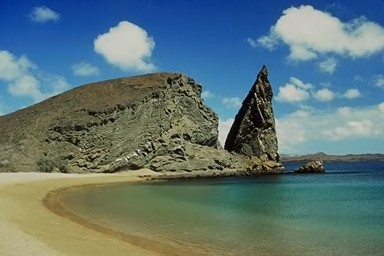
\includegraphics[width=.3\linewidth]{\detokenize{figuras/geracao/saliency-a.png}}
    }
    \subfloat[Original]{
      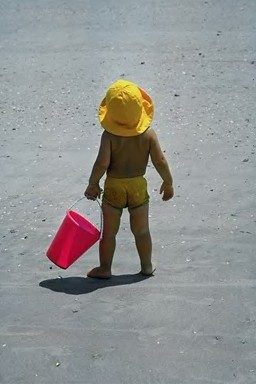
\includegraphics[width=0.3\linewidth]{\detokenize{figuras/geracao/saliency-b.png}}
    }
    \subfloat[Imagem artificial]{
      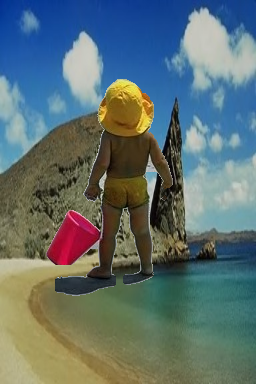
\includegraphics[width=.3\linewidth]{\detokenize{figuras/geracao/saliency-c.png}}
    }
  \end{center}
  \caption[Geração artificial utilizando uma mistura de duas imagens a partir da saliência da primeira imagem.]{Geração artificial utilizando uma mistura de duas imagens a partir da saliência da primeira imagem. \textit{Fonte:~Elaborado pela autora.}}
  \label{fig:gen:saliency}
\end{figure}

As operações aplicadas na imagem para extrair a região mais saliente são: segmentação pelo método SLIC; rotulação por conectividade; \textit{threshold de OTSU}; e operações morfológicas. O Algoritmo~\ref{alg:saliency} apresenta os passos para o cálculo do \textit{background} e \textit{foreground}.

\vspace{0.5cm}
\begin{algorithm}[!htbp]
  \caption{Geração artificial: mistura saliente}
  \label{alg:saliency}
  \SetAlgoLined
  \Entrada{
    \begin{itemize}
      \item[] Imagem colorida $I$ em formato RGB
      \item[] Imagem colorida $I_2$ em formato RGB
    \end{itemize}
  }
  \Saida{Imagem gerada $G$}

  $I_{\text{rotulada por segmento}} \gets SLIC(I)$\;
  $I_{\text{mapa de saliência}} \gets \text{rotulação por conectividade}(I_{\text{rotulada por segmento}})$\;
  $I_{threshold} \gets OTSU(I_{\text{mapa de saliência}})$\;
  $I_{morfologica} \gets \text{abertura e dilatação} (I_{threshold})$\;
  $I_{foreground} \gets \text{aplica máscara}(I_{morfologica}, I) $\;
  $I_{morfologica} \gets \text{oposto}(I_{morfologica})$\;
  $I_{background} \gets \text{aplica máscara}(I_{morfologica}, I_2) $\;
  $G \gets I_{background} + I_{foreground}$\;
\end{algorithm}
\vspace{0.5cm}

\begin{description}
  \item[Parâmetros e suas variações] Assim como no método anterior, os parâmetros são relacionados ao tamanho do elemento estruturante para a abertura e dilatação e estão fixos.

  \item[Limitações] Não é garantido que o algoritmo de saliência consiga extrair
  a melhor região, ou mesmo que sempre haja uma região saliente.

  \item[Métodos relacionados] Assemelha-se à mistura por \textit{thresholds}.

  % \item[Visualização]
\end{description}
%%%%%%%%%%%%%%%%%%%%%%%%%%%%%%%%%%%%%%%%%%%%%%%%%%%%%%%%%%%%%%%%%%%%%%%%%%%%%%%%
\section{Composição}

Essa geração pretende compor informações de diversas imagens em uma única. Assim é feito um mosaico com várias imagens, conforme pode ser visto na  Figura~\ref{fig:gen:composition}. Para cada quadrado a ser preenchido, sorteia uma imagem do conjunto de treinamento; realiza uma operação de borramento, aguçamento, mistura ponderada ou SMOTE visual; e adiciona essa imagem no quadrado respectivo. Os passos para tal composição estão descritos no Algoritmo~\ref{alg:composition}.

% Se as imagens possuem um elemento centralizado, essa geração pode resultar em uma imagem de um objeto que parece uma mutação dos objetos centrais, conforme pode ser visualizado na Figura~\ref{}.
%
% \meutodo{figura da mistura central}

\begin{figure}[!htbp]
  \begin{center}
    \centering
    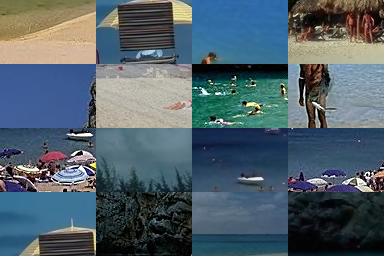
\includegraphics[width=0.6\linewidth]{\detokenize{figuras/geracao/composition.png}}
  \end{center}
  \caption[Geração artificial utilizando uma composição de imagens.]{Geração artificial utilizando uma composição de imagens. \textit{Fonte:~Elaborado pela autora.}}
  \label{fig:gen:composition}
\end{figure}


\vspace{0.5cm}
\begin{algorithm}[!htbp]
  \caption{Geração artificial: composição}
  \label{alg:composition}
  \SetAlgoLined
  \Saida{Imagem gerada $G$}
  \Enqto{total < \text{número de quadrados $q$}}{
  $I \gets \text{imagem aleatória do conjunto de treinamento}$\;
  $\text{operação} \gets 1 + (rand() \% 3 )$\;
  \Selec{\text{operação}} {
  \uCaso{1} {
  $I \gets borramento(I)$\;
  }
  \uCaso{2} {
  $I \gets \text{mistura ponderada}(I)$\;
  }
  \uCaso{3} {
  $I \gets \text{aguçamento}(I)$\;
  }
  \uCaso{4} {
  $I \gets \text{visual SMOTE}(I)$\;
  }
  }
  $x \gets \text{posição aleatória em x de I}$\;
  $y \gets \text{posição aleatória em y de I}$\;
  $qx \gets \text{posição atual para o quadrado em x de G}$\;
  $qy \gets \text{posição atual para o quadrado em y de G}$\;
  $G(qx, qy) \gets I(x,y)$\;
  $total++$\;
  }
\end{algorithm}
\vspace{0.5cm}

\begin{description}
  \item[Parâmetros e suas variações] O parâmetro $q$ controla quantos quadrados serão criados na nova imagem. Nesta pesquisa foram realizados testes com 4 e 16 quadrados.

  \item[Limitações] O término brusco de uma imagem para início da outra, ao formar a grade de imagens, tem efeitos colaterais de inserção de textura que não excedam a vantagem de compor uma mesma imagem com várias cores, texturas e formas das imagens originais.

  \item[Métodos relacionados] Fazer uma composição de imagens em quadrantes pode estar relacionado com a composição ao utilizar saliência.

  % \item[Visualização]
\end{description}
%%%%%%%%%%%%%%%%%%%%%%%%%%%%%%%%%%%%%%%%%%%%%%%%%%%%%%%%%%%%%%%%%%%%%%%%%%%%%%%%
% \item \underline{Redes neurais}: por representarem o estado da arte da classificação, reconhecimento e localização de objetos, as redes neurais de convolução são estudadas. Pretende-se utilizar a análise dos resultados do seu treinamento para identificar as características relevantes em imagens. Já as máquinas de Boltzmann restritas são redes neurais mais simples, portanto convenientes para a verificação da relevância de uma imagem para o aprendizado.
%  \item[Implementação:] a biblioteca \-OpenCV \cite{Intel2010} será utilizada para as funções gerais de carregar, processar, salvar e classificar imagens. A linguagem de programação para utilizar esta biblioteca e na qual esta pesquisa está sendo implementada é C++. Para a geração de gráficos das medidas estatísticas a linguagem de programação Python é utilizada. O código está disponível em \url{https://bitbucket.org/moacirponti/imagefeatureextraction/overview}.
%  \item[Bases de imagens:] considerando que os objetivos propostos possuem um viés genérico, os experimentos vão ser realizados em diversas coleções de imagens com o objetivo de estabelecer ou refutar as hipóteses levantadas.
%
%  Os resultados preliminares foram obtidos utilizando a base de imagens COREL\footnote{Disponível em http://wang.ist.psu.edu/docs/related/}, composta por fotografias que representam as classes: tribos africanas, praia, construções, ônibus, dinossauros, elefantes, flores, cavalos, montanhas e tipos de comidas. São 10 classes balanceadas com 100 imagens cada. Para fins de exemplificação, foram selecionadas imagens que representam essas classes na Figura \ref{fig:corel}.
%
%  \begin{figure}[hbpt]
%  \begin{center}
%    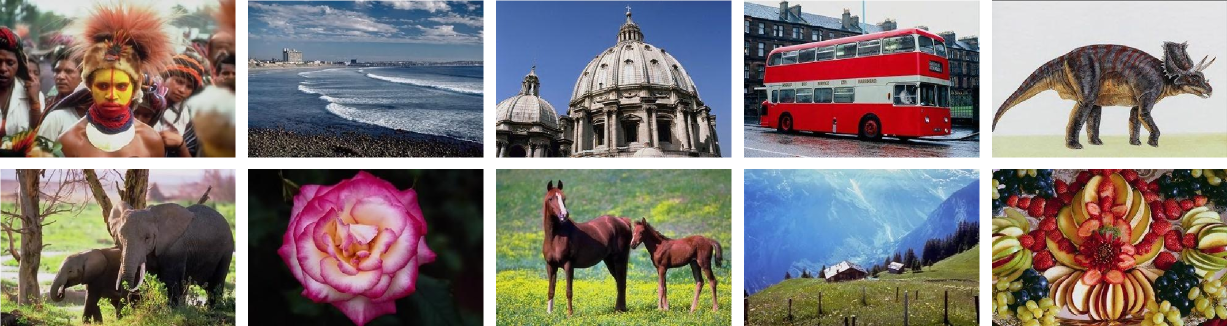
\includegraphics[width=1\linewidth]{\detokenize {figuras/exemplos_corel.png}}
%  \end{center}
%   \caption[Base de imagens COREL-1000.]{Base de imagens COREL-1000 utilizada. Estão representadas as 10 classes da base. \textit{Fonte: Elaborado pela autora.}}
%  \label{fig:corel}
% \end{figure}
%
%
%  \item[Experimentos:] serão realizados diversos experimentos direcionados a explorar as etapas de pré-processamento, para melhorar a acurácia da classificação de bases de imagens. Como entrada são utilizadas imagens originais provenientes de diversas coleções disponíveis na literatura. Como resultado, serão calculadas medidas estatísticas da classificação dessas coleções após a alteração dessas imagens com os métodos de realce de características relevantes.
%
%  \item[Análise dos dados:] os experimentos realizados irão resultar em medidas estatísticas da classificação. A análise irá comparar a classificação das imagens originais com aquelas tratadas pelo método proposto. Ainda, o método de rebalanceamento de classes será comparado com técnicas disponíveis na literatura, como o SMOTE.
%
% \item[Forma de avaliação:]
% Por fim, a \underline{distância de Mahalanobis} também pode ser utilizada: antes e depois da geração artificial de imagens, calcular a distância entre a média das classes e a variância dentro das classes \cite{mahalanobis2000}. Ela se baseia na correlação entre as variáveis e pode ser definida por
% \begin{equation*}
%   D_m(x_i) = \sqrt{(x_i - \mu)C^{-1}(x_i-\mu)^T},
% \end{equation*}
% \noindent onde $x_i$ é um vetor de valores, $\mu$ a média e C a matriz de covariância.
%
% \end{description}
%
% %-------------------------------------------------------------------------------
% \section{Resultados esperados}
% \label{sec:resultados}
%
% Os resultados esperados são relacionados às áreas de \textbf{processamento de imagens e reconhecimento de padrões}. Espera-se obter uma comprovação das hipóteses levantadas por essa pesquisa. Os resultados são esperados em duas vertentes:
%
% \begin{enumerate}
%  \item \textit{Pré-processamento} de imagens que caracterizem melhor aspectos de suas classes, aumentando a variância entre as classes quando comparado com as imagens originais.
%  \item \textit{Geração artificial de imagens} de classes minoritárias de forma a compensar o desbalanceamento natural das bases de dados.
% \end{enumerate}
%
% Em ambos os casos pretende-se melhorar a classificação, validando-a através do cálculo da medida-F1. A análise das características aprendidas por uma rede neural de convolução será realizada ao executar o treinamento com bases específicas que destaquem propriedades como cor, textura e forma. Além disso, os resultados serão obtidos a partir da escolha de quais imagens adicionam informação ao conjunto de treino. As redes RBM serão utilizadas para este fim. Bases naturalmente não balanceadas serão testadas e seus resultados avaliados.


%-------------------------------------------------------------------------------
\section{Considerações finais}

Esse capítulo descreveu como o rebalanceamento é realizado, através da geração de imagens artificiais para a classe (ou classes) minoritárias, utilizando-as assim para o treinamento. Os métodos para gerar tais imagens foram apresentados e exemplificados. Foram também descritos os algoritmos, parâmetros utilizados, limitações e métodos relacionados a cada um destes algoritmos. Os resultados da utilização dos métodos descritos neste capítulo estão no Capítulo~\ref{cap:resultados-geracao}.

% A proposta desta pesquisa foi apresentada, descrevendo a sua metodologia. Foi dado destaque aos resultados esperados e à forma de avaliação, descrevendo as medidas estatísticas a serem utilizadas. O cronograma previsto para a realização deste mestrado foi destacado, elencando as atividades e suas respetivas durações. O próximo capítulo apresentará os resultados preliminares.
